\documentclass[12pt,twocolumn]{article}
\usepackage[T1]{fontenc}
\usepackage{graphicx}
\usepackage{tabularx}
\usepackage{amsmath,amsthm,amssymb}
%\usepackage{esvect}
\usepackage[left=1cm,right=1cm,top=2cm,bottom=2cm]{geometry}
%\renewcommand*{\familydefault}{\sfdefault}
\title{\vspace{-2.5em}Transient Diffusion}
\author{Christopher Pattison}
\date{}
\begin{document}
\maketitle
\section*{Introduction}

\section*{Derivation}
The transient conduction equation \eqref{eq:transcond} was modeling using the Finite Volume Method.
\begin{equation}\label{eq:transcond}\nabla\cdot k\nabla T + q = \rho C_P\dot T\end{equation}
In addition to integrating over the control volume, the timestep is also integrated over.
\begin{equation}\label{eq:fvmtranscond}\int_{\Delta t}\int_V( \nabla\cdot k\nabla T + q - \rho C_P\dot T)dVdt\end{equation}
If $T_P$ and $q_P$ are presumed to predominate the control volume and $\rho C_P$ is constant, by the divergence theorem equation \eqref{eq:fvmsimpl} is obtained.
\begin{equation}\label{eq:fvmsimpl}\sum\limits_{\partial V} k\nabla T \cdot \hat n_i + q \Delta x - \rho C_P \dot T \Delta x\end{equation}
\begin{equation}\label{eq:fvmfinal}\left(\sum\limits_{\partial V} k\nabla T \cdot \hat n_i + q \Delta x\right)^{k+m} - \rho C_P (T_{k+1} - T_k) \frac{\Delta x}{\Delta t}\end{equation}
The gradient descretization is applied in equation \eqref{eq:fvmfinal}. 
Depending on the selection of $m$ the result is Implicit Euler ($1$), Explicit Euler ($0$), or Crank-Nicolson ($\frac{1}{2}$).

\begin{figure}
\includegraphics[width=\columnwidth]{plot/sol.png}
\footnotesize{\caption{Constant heat flux solution}}
\end{figure}

\section*{Transient Solver Performance}
Implicit Euler being unconditionally stable performed extremely well although there was an associated computational cost with solving a linear system.
\paragraph{}
Explicit Euler can be put into the form of equation \eqref{eq:expleuler}.
\begin{equation}\label{eq:expleuler}\{T\}^{k+1} = ([A]\{T\}^k + \{b\})\frac{\Delta t}{\rho C_P \Delta x}\end{equation}
This allows for extremely quick timestepping since only matrix multiplication needs to be carried out. 
However, the stable timestep was extremely low.
\paragraph{}
Since Crank Nicolson is second order, as the time step decreases, Crank Nicolson becomes much more accurate. 
Notably, the instability of Explicit Euler means that the stable timestep is somewhat low

\section*{Manufactured Solutions}
The Method of Manufactured Solutions can be applied.
With $T=\sin x \cos t$ the source term in equation \eqref{eq:mansol1} is obtained.
\begin{equation}\label{eq:mansol1}S = (k\cos t - \sin t)\sin x - q\end{equation}
Error can be quantified by equation \eqref{eq:error}
\begin{equation}\label{eq:error}\epsilon \propto \sqrt{\frac{1}{N} \sum\limits_{i,j}^N (\hat T (x_i,t_j) - \tilde T_{i,j})^2}\end{equation}
\begin{equation}\epsilon(h,\Delta t) = O(h^2,\Delta t^n)\end{equation}
\paragraph{} Error is some function of both grid spacing $h$ and timestep $\Delta t$. Since the special discretization is second order, the error should go down with the square of $h$ if $\Delta t = 0$.
\paragraph{} If Implicit or Explicit Euler is used, then $n=1$ and the error should be proportional to $\Delta t$ if $h=0$.
\paragraph{} Notably, error seems to be converging to a value above zero. This could be due to spacial error since it is non-zero.

\section*{Improvement}
Since error is cummulative in the time domain and dependant on the length of time, a better characterization of error is needed.
One option could be to normalize the error by the simulation time.
\begin{equation}\epsilon = \frac{O(h^2,\Delta t)}{t}\end{equation}
This would give an error that is less dependant on the simulation time. Which may make error somewhat less dependant on time.
\begin{figure}
\includegraphics[width=\columnwidth]{plot/mansol.png}
\footnotesize{\caption{Manufactured solution}}
\end{figure}

\begin{figure}
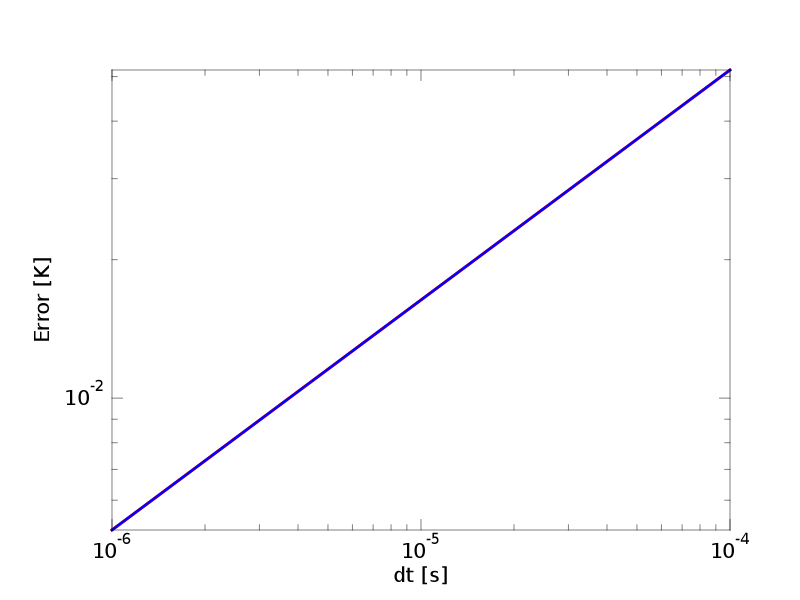
\includegraphics[width=\columnwidth]{plot/error.png}
\footnotesize{\caption{Crank-Nicolson and Euler Implicit Global Error}}
\end{figure}

\begin{figure}
\label{fig:timeerrror}
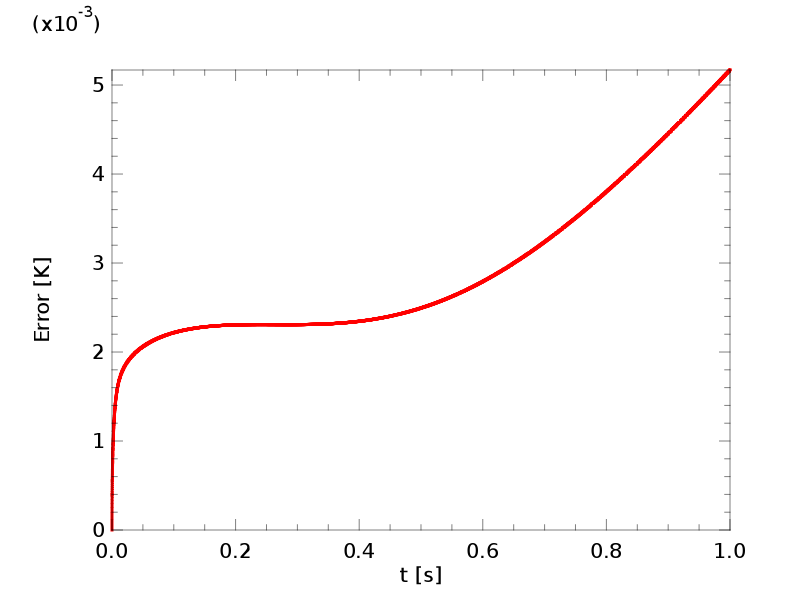
\includegraphics[width=\columnwidth]{plot/timeerror.png}
\footnotesize{\caption{Cumulative Error}}
\end{figure}

\end{document}

